\documentclass[10pt]{article}
\usepackage{graphicx}
\usepackage[margin=1.5cm]{geometry}
\usepackage{amsmath}
\def\brcurs{{\mbox{$\resizebox{.16in}{.08in}{
\includegraphics{BoldR}}$}}}
\def\rcurs{{\mbox{$\resizebox{.16in}{.08in}{
\includegraphics{ScriptR}}$}}}

\begin{document}
\twocolumn

\title{Thursday Warm-up: Electric Fields in Matter}
\author{Prof. Jordan C. Hanson}

\maketitle

\section{Memory Bank}

\small

\begin{itemize}
\item \textbf{Bound surface charge density}, given a polarization $\mathbf{P}$:
\begin{equation}
\sigma_{\rm b} = \mathbf{P} \cdot \hat{\mathbf{n}}
\end{equation}
\item \textbf{Bound volume charge density}, given a polarization $\mathbf{P}$:
\begin{equation}
\rho_{\rm b} = -\nabla \cdot \mathbf{P}
\end{equation}
\item \textbf{Cartesian and cylindrical unit vectors}:
\begin{align}
\hat{\mathbf{x}} &= \cos\phi \hat{\mathbf{s}} - \sin\phi \hat{\boldsymbol{\phi}} \\
\hat{\mathbf{y}} &= \sin\phi \hat{\mathbf{s}} + \cos\phi \hat{\boldsymbol{\phi}} \\
\hat{\mathbf{z}} &= \hat{\mathbf{z}}
\end{align}
\item \textbf{Divergence in cylindrical coordinates}:
\begin{equation}
\nabla \cdot \mathbf{v} = \frac{1}{s}\frac{\partial}{\partial s}(s v_s) + \frac{1}{s}\frac{\partial v_\phi}{\partial \phi} + \frac{\partial v_z}{\partial z}
\end{equation}
\item \textbf{The electric displacement}:
\begin{equation}
\mathbf{D} = \epsilon_0 \mathbf{E} + \mathbf{P}
\end{equation}
\item \textbf{Gauss' Law for electric displacement}:
\begin{equation}
\oint \mathbf{D} \cdot d\mathbf{a} = Q_{\rm f,enc}
\end{equation}
\end{itemize}

\begin{figure}
\centering
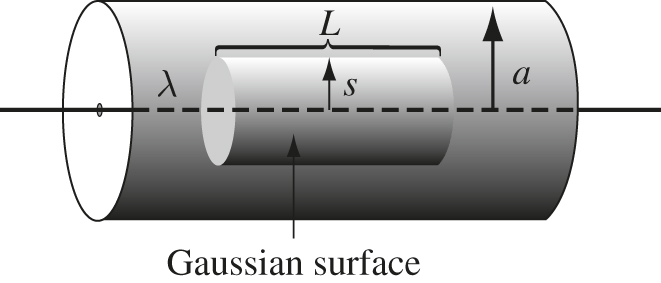
\includegraphics[width=0.4\textwidth]{figures/4_17.jpg}
\caption{\label{fig:1} A charge distribution with density $\lambda$ [C m$^{-1}$] is embedded in a dielectric material with $\mathbf{P} = (k/s) \hat{\mathbf{s}}$.}
\end{figure}

\section{Gauss' Law Review}

\begin{enumerate}
\item Consider Fig. \ref{fig:1}.  Imagine that $\mathbf{P} = 0$ in the region surrounding the linear charge distribution. (a) Calculate $\mathbf{E}$. (b) Calculate $V(\mathbf{r})$. \\ \vspace{4cm}
\end{enumerate}

\section{Polarization and Bound Charge}
\label{sec:3}

\begin{enumerate}
\item Consider Fig. \ref{fig:1}.  Given $\mathbf{P} = (k/s) \hat{\mathbf{s}}$, calculate (a) the bound volume charge density, $\rho_{\rm b}$, and (b) the bound surface charge density, $\sigma_{\rm b}$. \\ \vspace{2.5cm}
\end{enumerate}

\section{The Electric Displacement}

\begin{enumerate}
\item (a) Write down the differential form of Gauss' Law, and substitute $\rho = \rho_{\rm f} + \rho_{\rm b}$. (b) Substitute $\mathbf{P}$ for $\rho_{\rm b}$ using the definition in the Memory Bank. (c) Solve for $\rho_{\rm f}$. (d) Identify $\mathbf{D}$. What are the units of $\mathbf{D}$? \\ \vspace{1cm}
\item (a) Calculate the \textit{electric displacement} for the system in Fig. \ref{fig:1}, inside the dielectric cylinder.  First, use Gauss' Law for $\mathbf{D}$.  Next, find $\mathbf{E}$ using $\mathbf{P}$ and $\mathbf{D}$. (b) Using the result for $\sigma_{\rm b}$ obtained  in Sec. \ref{sec:3}, find the field outside the cylinder using Gauss' Law. (c) Find $\mathbf{D}$ outside the cylinder using Gauss' law, and check that it is consistent with (b). \\ \vspace{4cm}
\item Suppose the polarization with a volume below the xy-plane is $\mathbf{P}=P\hat{\mathbf{z}}$. (a) Find $\sigma_{\rm b}$ and $\rho_{\rm b}$.  (b) Find $\mathbf{D}$ and $\mathbf{E}$ in the region above the plane. (c) How would you conceive of $\mathbf{E}$ and $\mathbf{D}$ for a capacitor fill with a dielectric material?
\end{enumerate}

\end{document}
